\documentclass[12pt]{article}
\usepackage[margin=1in]{geometry} 
\usepackage{amsmath,amsthm,amssymb,amsfonts}
\usepackage{graphicx}
\usepackage{float}
\newcommand{\N}{\mathbb{N}}
\newcommand{\Z}{\mathbb{Z}}
\newenvironment{problem}[2][Problem]{\begin{trivlist}
		\item[\hskip \labelsep {\bfseries #1}\hskip \labelsep {\bfseries #2.}]}{\end{trivlist}}
{\newpage\renewcommand{\thepage}{\arabic{page}}\setcounter{page}{1}}
\usepackage{natbib}
\usepackage{url}
\begin{document}
	\title{Senior Thesis Mini-Proposal}
	\author{Tyrone Zhang}
	\maketitle
	\section{Abstract}
	Princeton’s climate is temperate, with no dry season, and a hot summer, which means that we should see precipitation events spread out throughout a year. With the weather data collected on top of guyot hall, I believe that we will be able to demonstrate that the precipitation events do follow the poisson distribution, as well as being able to use humidity, air pressure, and air temperature to be able to predict rainfall in the future. 
	
	\section{Introduction}
	The Climatology of Princeton is clearly one that belongs to the mid-latitudes, which is characterized by having four seasons that results in having a large variation in temperature throughout a year. In terms of the average calculated between 1981 and 2010, Princeton gets an average of 48.27 inches (1227 mm) of precipitation annually, and the precipitation distribution throughout the year is fairly even, with less precipitation in the winter (PRISM Project).  According to the Köppen–Geiger Climate Classification, Princeton, NJ lies in the classification Cfa, which denotes a temperate climate, with no dry season, and hot summers defined as reaching 22 degrees Celsius or higher \cite{Peel2008}. Princeton having no dry season means that precipitation should be well spread throughout the year. The weather station that I am getting my data from is a Vaisala weather transmitter WXT530 series. It measures the six weather parameters of air pressure, temperature, humidity, rainfall, wind speed ,and wind direction. The rainfall is measured using an acoustic Vaisala RAINCAP Sensor, which helps avoid the complications of flooding, wetting, and evaporation losses \cite{Vaisala}. One of the good aspects in using machine learning for weather forecasting over numerical weather models is that machine learning costs much less computationally, which allows outperforms many non-numerical weather models \cite{Scher}. 
	
	\begin{figure}[H]
		\centering
		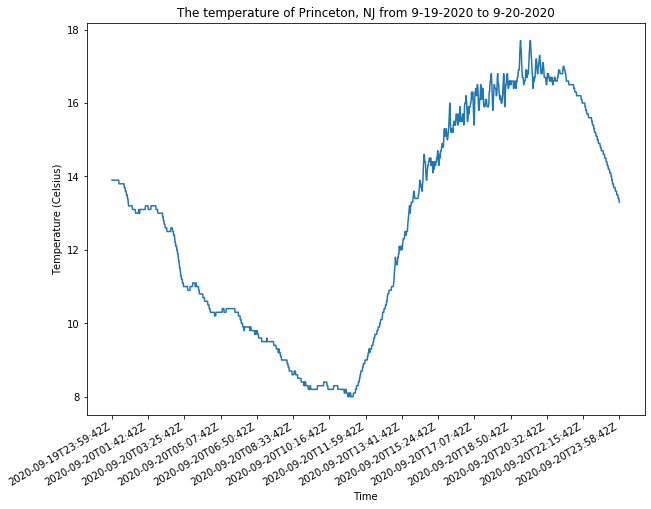
\includegraphics[width=130mm]{Figures/Day_temp_profile.png}
		\caption{This is the temperature profile on Day 264 of year 2020. The data is from 8 PM on September 19th to 8 PM on September 20th. One can clearly see the diurnal cycle, as the temperature drops during the night until the sun rises. Then the temperature rises until sun down. }
	\end{figure}
	\section{Objectives and Methods}
	Some objectives for the senior thesis is to use machine learning to predict when precipitation occurs, given a few of the variables that are also measured from the weather station. Before using Machine learning to try to predict precipitation, I will be examining the nature of the precipitation data, namely how are these precipitation events occurring, what is the intensity of each precipitation event, how to define a precipitation event, as there are cases in which we end up having one minute rain events which is really small. Some insight comes from Eagleson, who used Poisson distribution as a model to look at precipitation events \cite{Eagleson}. Similarly, Heat waves are subjected to similar analysis, as to how to define a heat wave and what cut off duration and intensity should be defined to meet a criteria of a heat wave. Once these criterias are determined, I will start using different machine learning methods to try to predict precipitation events and heat waves. Some methods that have been used to predict future weather conditions have used neural networks with machine learning to generate predictions for the future. 
	
	\section{Budget Justification}
	As of right now, I do not have any expenses. This is because the data that I am going to analyze and use in this project is accessible online for free, as Professor Simons posts the data online. Furthermore, using python is free and thus there are no expenses related to that. As I am not traveling anywhere but my home, I don’t expect any transportation expenses as well as any expenses related to a research laboratory.  
	
	%--References
	\small
	\renewcommand{\bibsep}{0em}
	
	\renewcommand{\bibname}{References}
	\bibliographystyle{Latex/gji}
	\bibliography{mini_ref}
\end{document}